\chapter{Part Selection
\index{Chapter!Part Selection}
\index{Part Selection}
\label{Part Selection}}

\begin{figure}[H]
  \centering
  \scalebox{.8}{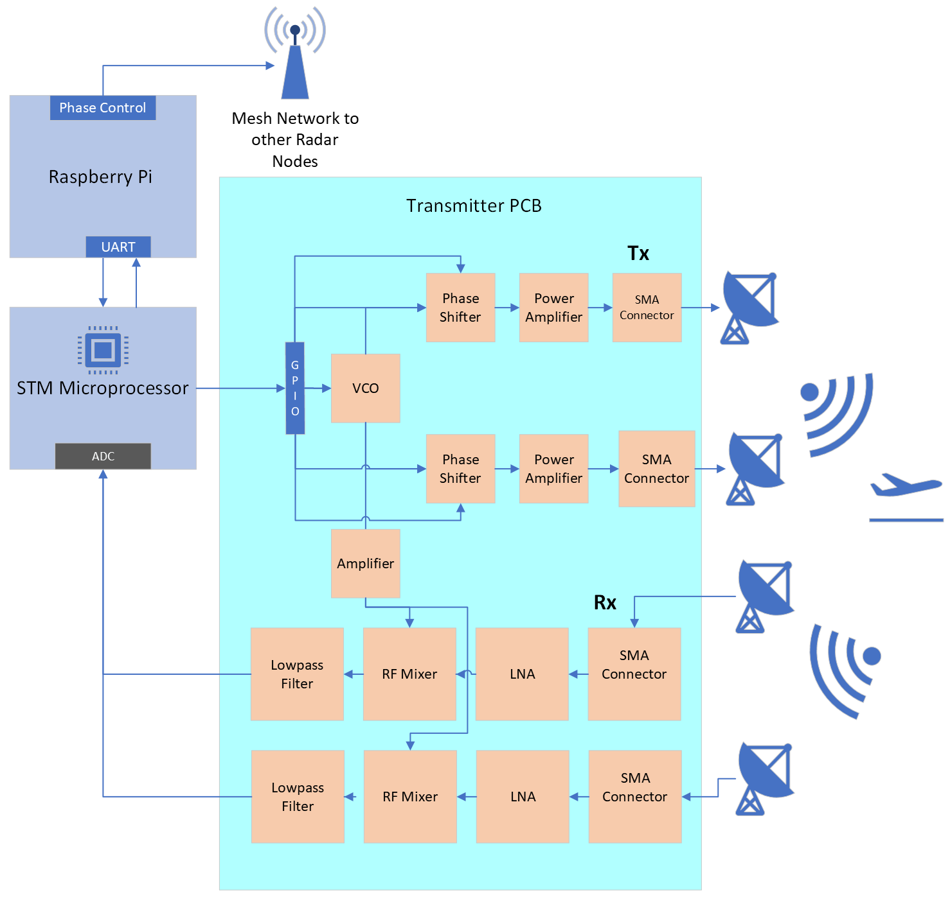
\includegraphics{Diagrams/overview.png}}
\caption{Architecture Overview}
\label{img:projoverview}
\end{figure}

In this chapter, we will go through the architecture of the PCB and show what parts we picked and what purposes they serve.
Figure \ref{img:projoverview} shows the overall architecture of the project.

\section{Voltage Controlled Oscillator (VCO)}
The first step in creating a radar is signal synthesis. You essentially need to create an alternating current signal that can
go through your antenna and radiate out into the air. To reiterate from Chapter \ref{Radar Theory}, higher frequency signals are
important for a better radar resolution, and so it is desired to have a signal that is high in frequency. Naively, at the
beginning of this project we thought we could use a 16 bit DAC to synthesize our signal but after finding out its max clock rate 
was 1 MHz, we realized a DAC was not fit for this. All we needed was something that could create a simple sinusoid at a very
high frequency.

Voltage Controlled Oscillators (VCO) do just this. They take in a "tuning voltage" which corresponds to a certain frequency
of sinusoid which it will output. The circuitry for this is beyond me, but for a good overall guide on VCOs you can check out
DigiKey's article \href{https://www.digikey.com/en/articles/the-basics-of-voltage-controlled-oscillators-vcos}{here}.

Now that we knew how to synthesize our signal, it was important to find a good VCO that had a high output bandwidth. Whatever
bandwidth the VCO has will impact what parts we can get in the other stages of the RF chain since these must be within the VCOs
operating regions. 

\begin{figure}[H]
    \centering
    \scalebox{.7}{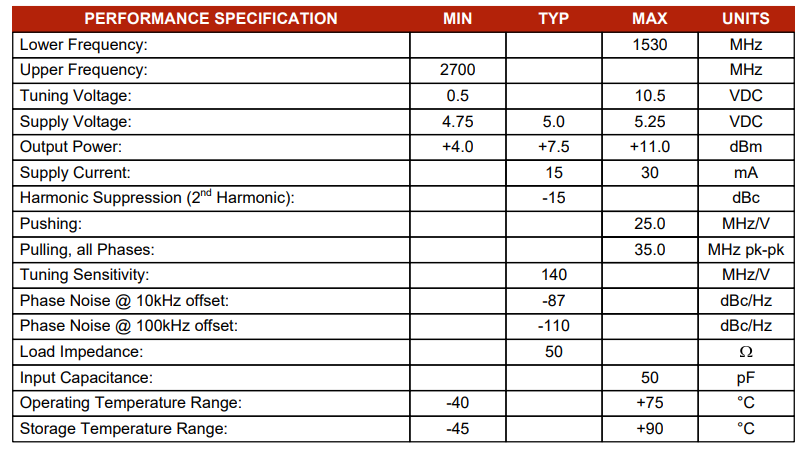
\includegraphics{DatasheetImages/vcotable.png}}
    \caption{VCO Datasheet Table}
    \label{img:vcotable}
\end{figure}
\begin{figure}[H]
    \centering
    \scalebox{.7}{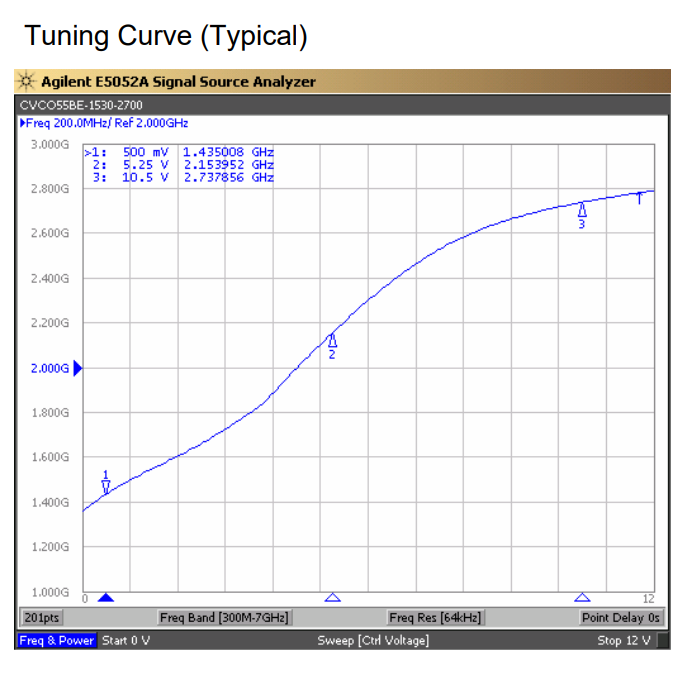
\includegraphics{DatasheetImages/vcotuningtable.png}}
    \caption{Tuning Voltage Graph}
    \label{img:tuninggraph}
\end{figure}

We chose a VCO from Crystek which can be found on Digikey \href{https://www.digikey.com/en/products/detail/crystek-corporation/CVCO55BE-1530-2700/1644030}{here}.
Looking at the specifications table in Figure \ref{img:vcotable}, some good things to look for are first and foremost the frequency
range of the part. It goes from about 1.5-2.7 GHz, which is a pretty wide range and would support a lot of other parts as it also
covers the Wi-Fi band. The second thing to look for is output power. The output power can be a constraint for other parts, since they
might have a absolute limit on their input power, and it is useful to know the output power for finding out how strong your signal will be
once it propogates out of your antenna. Here we can see the output power is around 7.5 dBm, and this will be split four ways. 
Decibels are a logarithmic scale, so we cannot just divide by four but instead use a decibel calculator like \href{https://noisetools.net/decibelcalculator}{this one}.

Now, another key metric is the tuning voltage. Luckily, this Crystek provides a tuning voltage graph found in Figure \ref{img:tuninggraph}
that shows us how the output frequency changes with changes in the tuning voltage. One observation is that it is not linear, meaning
our ramp voltage will not result in a true linear ramp in frequency. Another observation is that our chosen frequency of 1.8 GHz is
around 3.5 volts following the graph. Our STM board that will generate the ramp voltage can by default only go to 3.3 volts, but we
found a workaround to go to 5 volts which allowed us to stick with our decided center frequency.

\section{Power Divider}
As mentioned before, we want to divide the VCO's signal four ways because want it to go to two phase shifters, and two mixers.
At first we thought it was as simple as having one wire split into four, but as we will go over in Chapter \ref{PCB}, impedence
matching is very important in RF circuits. To put it simply, impedance matching ensures that no power is reflected, and this is
important because reflected power means distortions in the signal and power loss. That means we needed a power splitter meant for
splitting an RF signal without causing reflected power. There is not much of note with the part we used which can be found 
\href{https://www.mouser.com/ProductDetail/Mini-Circuits/WP4P1%2B?qs=Imq1NPwxi77kWybHhilv%2Fg%3D%3D}{here}. The main thing is that
it contains the frequency of 1.8 GHz we want to use.

\section{Phase Shifter}
Two of the power dividers split paths will go into phase shifters. The phase shifters are used to make our phased array
of antennas as explained in Chapter \ref{Radar Theory}. They are able to change the phase (add time delay), to the signal 
so that when they propogate through the air they can construct and destruct. The phase shifters we chose can be found
\href{https://www.digikey.com/en/products/detail/psemi/PE44820B-X/5822957}{here}. These are digital phase shifters that have 256
different phases it can apply to the signal. They have a parallel or serial interface we can use to transmit 8 bit words That
will alter the phase of our signal. The interface and its timing diagrams will be explained more in detail in Chapter \ref{Digital Processing}.
All we need to know is that the bandwidth that the chip supports contains 1.8 GHz.

\section{Power Amplifier}
\begin{figure}[H]
  \centering
  \scalebox{.6}{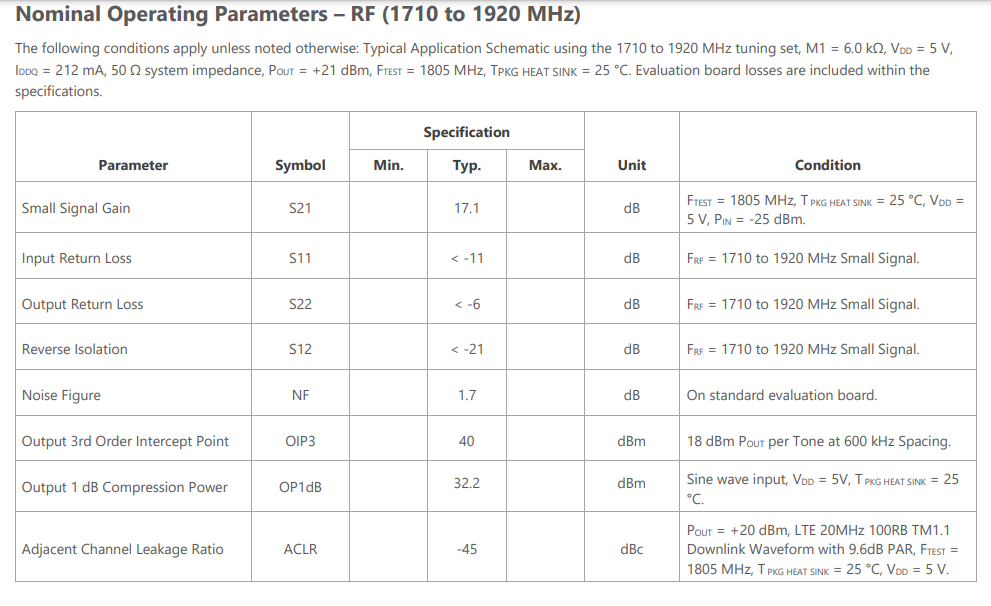
\includegraphics{DatasheetImages/poweramptable.png}}
  \caption{Power Amplifier Table}
  \label{img:poweramptable}
\end{figure}
At this point after the VCO and phase shifter, we want the RF signal to propogate through the air. However, according to the
radar range equation the power of the signal when attenuating through the air attenuates at a power of four which is a lot.
Therefore, we need to make sure our signal is powerful enough to go pretty far. So, we use an RF power amplifier to amplify the
signal. We chose a part from GuerillaRF which can be found \href{https://www.mouser.com/ProductDetail/Guerrilla-RF/GRF5112?qs=ulEaXIWI0c%252Bti188Qa1Now%3D%3D}{here}.
Looking at the table in Figure \ref{img:poweramptable}, we can see some key metrics when looking at power amplifiers. First,
of course we want to make sure it has a bandwidth that supports our chosen frequency of 1.8 GHz. Second, we want to look at the
small-signal gain and Output 1 dB Compression Point or OP1dB. The small-signal gain is the ideal gain that can be reached with a 
low power signal, and is listed as 17.1 dB. The OP1dB is a metric we did not know about and were thankful to find it. With most amplifiers,
gain operates linearly meaning whatever power your input signal is you just add the gain of the amplifier and this will be the resulting power of the signal.
However, at a certain point the amplifier saturates and does not operate linearly anymore, and will essentially cap-off its gain at
the OP1dB limit. For example, with the OP1dB being 32.2 dB, if I input a signal that was 30 dB I would expect a resulting signal of
47.1 dB but this would not be the case. The amplifier ceases to operate linearly after the 32.2 dB mark, and will both distort the signal
and output something weaker than expected. A lot of amplifiers will boast a high gain but have a low OP1dB, so this is definitely something to check for.

\section{Low Noise Amplifier}
\begin{figure}[H]
  \centering
  \scalebox{.7}{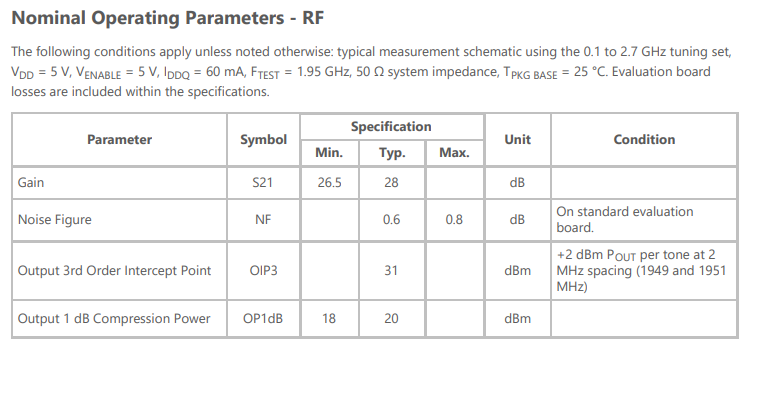
\includegraphics{DatasheetImages/lnatable.png}}
  \caption{Low-Noise Amplifier Table}
  \label{img:lnatable}
\end{figure}

This is the first part that will be placed in the receiver RF chain. According to the Friis equation in Chapter \ref{Radar Theory},
the first stage in the receiver RF chain matters a lot for the noise figure of your system. Therefore, we wanted to find a part
with a low noise figure and high gain, as this will impact our SNR the most. Low noise amplifiers are made for this exact purpose,
where they amplify a small signal with very low noise. The part we chose was \href{https://www.mouser.com/ProductDetail/Guerrilla-RF/GRF2133W?qs=ulEaXIWI0c%2FXgAPwqRmr2A%3D%3D}{this},
which is made by GuerillaRF. By examining the table in Figure \ref{img:lnatable}, we can see that it has a gain of 28 dB,
and a noise figure of .6 dB. We also can look at the OP1dB which has a figure of 20 dB. Since the LNA will be amplifying a signal
straight from an antenna, the signal will be super weak and there is a low likelihood it will reach the OP1dB.

\section{Mixer/LO Amp}